\documentclass[../main.tex]{subfiles}

\begin{document}

% -------------------------------------------
\subsection{Manual de usuario.}\label{Manual de usuario}
La prueba de concepto requiere tener instalada la distribución de \textbf{Docker} adecuada al sistema operativo del dispositivo en el que se quiere ejecutar. De esta manera, únicamente se necesita que el usuario introduzca en una terminal abierta desde el directorio raíz del proyecto (donde se encuentra el archivo docker-compose.yml) el siguiente comando:

\begin{lstlisting}[language=sh]
  docker compose up --build
\end{lstlisting}

\noindent Tras este paso, se generará la siguiente estructura de contenedores que se mantendrán activos aunque el usuario cierre la terminal y permitirán el correcto funcionamiento del sistema:

\begin{figure}[htbp]
    \centering
    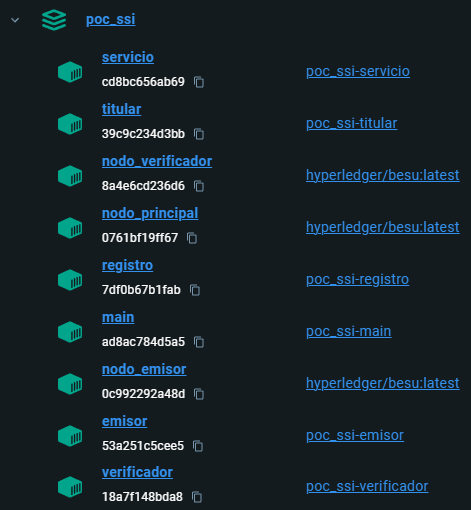
\includegraphics[width=0.57\linewidth]{images/design/contenedores.png}
    \caption{\textit{Visualización de los contenedores en Docker Desktop.}}
\end{figure}

\noindent Acudiendo a la dirección \textbf{http://127.0.0.1:5000} desde cualquier navegador, el usuario podrá seguir el transcurso descrito en la sección de la \hyperref[Prueba de concepto]{prueba de concepto}. También podrá acceder:

\begin{enumerate}
    \item Al contenido de las variables del Emisor, mediante la url: \quad  \textbf{http://127.0.0.1:5001}
    \item Al contenido de las variables del Titular, mediante la url: \quad \textbf{http://127.0.0.1:5002}
    \item Al contenido de las variables del Verificador, mediante la url: \quad \textbf{http://127.0.0.1:5003}
    \item Al contenido de las variables del Registro, mediante la url: \quad \textbf{http://127.0.0.1:5004}
    \item Al contenido de las variables del Servicio, mediante la url: \quad \textbf{http://127.0.0.1:5005}
\end{enumerate}

\begin{tcolorbox}[colback=gray!10!white, colframe=gray!50!black, title=Observación]\label{recomendacion}
Se recomienda refrescar las páginas de los actores involucrados cada vez que se efectúe un paso del flujo elegido. De esta manera, se podrá conocer el estado actual de cada componente de la \acrshort{SSI} y seguir su evolución durante la prueba de concepto.
\end{tcolorbox}

\noindent Una vez logrado el objetivo por el que se quiso ejecutar el sistema, se deberá terminar adecuadamente con la actividad de los contenedores. Esto se puede realizar de dos maneras:

\begin{itemize}
    \item Si la terminal sigue estando abierta, es suficiente con seleccionarla y pulsar las teclas CONTROL + C para así mandar una señal que terminará con los procesos en ejecución.
    \item Si por el contrario la hemos cerrado, hemos de realizar el siguiente comando:
\end{itemize}
\begin{lstlisting}[language=sh]
  docker stop $(docker ps -q)
\end{lstlisting}

\noindent Finalmente, resultaría correcto eliminar por completo todo elemento creado por el proyecto. Tras la ejecución de este comando desde cualquier terminal, se eliminará todo contenedor, volumen de datos e imagen creado por el sistema en el dispositivo del usuario.
\begin{lstlisting}[language=sh]
  docker compose -p poc_ssi down --rmi all -v
\end{lstlisting}

Alternativamente, puede realizarse este mismo proceso mediante la interfaz de usuario de Docker Desktop en caso de haberse instalado previamente (recomendado por su simplicidad).


\newpage
% -------------------------------------
\subsection{Características de diseño.}\label{Características de diseño}
Como puede haberse comprobado, el principal aspecto a destacar del sistema elaborado es su cómoda accesibilidad desde el navegador. Esto no fue considerado en primer instancia, ya que la visualización en terminal de las comunicaciones efectuadas y la posibilidad de acceder al propio contenedor parecían suficientes para monitorizar la prueba de concepto. 
\\

\noindent No obstante, el elevado número de actores y los frecuentes mensajes de los nodos que conforman la red Blockchain hacen demasiado engorrosa la visualización desde la terminal. Una solución a esta situación es acceder directamente a los registros (logs) de los contenedores para conocer su actividad individualmente, con el coste de perder la visión en conjunto del sistema. 
\\

\noindent Destacar que estas alternativas siguen estando disponibles aunque no son indispensables para realizar la función de monitorización, ya que gracias a determinadas \hyperref[Análisis sobre las tecnologías empleadas]{tecnologías} como \textit{Flask} es posible acceder desde el navegador mientras se realizan comunicaciones en segundo plano. 
\\

\begin{figure}[htbp]
    \centering
    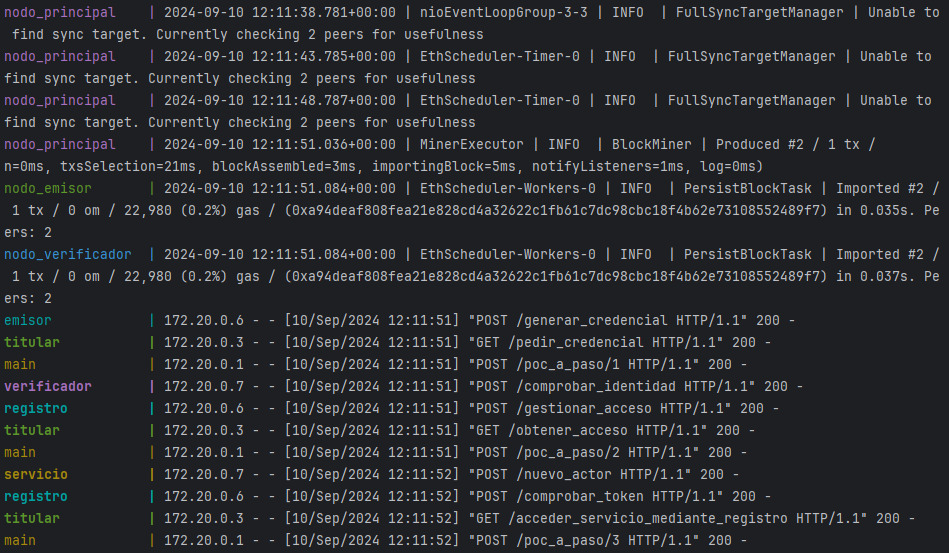
\includegraphics[width=1\linewidth]{images/design/comunicaciones.png}
    \caption{\textit{Ejemplo de comunicaciones entre contenedores durante los flujos.}}
\end{figure}

\newpage
\noindent Estos mensajes son enviados y recibidos mediante los endpoints de \textit{Flask} definidos en \textit{Python}. Por ejemplo, el siguiente fragmento de código es utilizado por el Titular para obtener la \acrshort{VC} creada por el Emisor, correspondiente al Paso 1 en cualquier flujo escogido (común a ambos). 

\begin{lstlisting}[language=Python]
@app.route('/pedir_credencial', methods=['GET'])  # Paso 1.
def pedir_credencial():
    # Construir la petición para el endpoint.
    datos_raw = {'did': titular.did}
    datos_bytes = json.dumps(datos_raw).encode('utf-8')
    peticion = titular.realizar_peticion(emisor_url + '/generar_credencial', datos_bytes, 'POST')

    try:
        # Obtener el contenido de la respuesta.
        respuesta = urllib.request.urlopen(peticion)
        credencial = str(respuesta.read().decode('utf-8'))

        # Realizar las acciones pertinentes.
        titular.guardar_credencial(credencial)

        # Comunicar la resolución definitiva.
        return jsonify({"Respuesta": "La credencial **SI** ha sido recibida y guardada."}), 200
    except urllib.error.HTTPError:
        return jsonify({"Respuesta": "La credencial **NO** ha sido recibida ni guardada."}), 400
\end{lstlisting}

\noindent En el sistema, todo endpoint comparte una estructura similar a la descrita ya que necesitan: 
\begin{itemize}
    \item Enviar algún tipo de información a otro/s actores para cumplimentar una petición.
    \item Recibir un mensaje con la respuesta obtenida distinguiendo los casos de éxito y fracaso.
    \item Comunicar el estado final de su petición a otro endpoint que haya llamado al actual. \\
    En el caso del Titular, es el cuasi-actor main el que requiere de confirmación.
\end{itemize}

\newpage
\noindent Con el objetivo de definir una distribución de los archivos creados en la prueba de concepto previa a la contenedorización de los actores, se diseña la siguiente estructura de carpetas:

\begin{itemize}
    \item En `\textbf{Actores}' se recogen un total de cinco subcarpetas asociadas a cada uno de los actores que participan en el sistema. En ellas se guardarán aquellos ficheros necesarios para la autonomía del mismo, como el Dockerfile o su \textit{Python} correspondiente.

    \item En `\textbf{Blockchain}' se definen los recursos requeridos por \textit{Besu} para el establecimiento de la red, como por ejemplo el genesis.json que describe su primer bloque o el propio contrato escrito en \textit{Solidity}, además de numerosos archivos de configuración de los nodos.  

    \item En `\textbf{Principal}' se encuentra el cuasi-actor main que supervisa el conjunto del sistema. Dentro de esta carpeta están vinculados los flujos a la batería principal de pruebas, la cual requiere de recursos web para visualizar la prueba de concepto en el navegador. 
\end{itemize}

\noindent Además, en el directorio raíz del proyecto (PoC\_SSI) se encuentra el docker-compose.yml del cual depende la correcta orquestación de los diferentes contenedores del sistema.
\\

\begin{figure}[htbp]
    \centering
    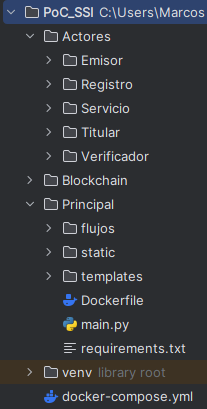
\includegraphics[width=0.3\linewidth]{images/design/proyecto.png}
    \caption{\textit{Estructura de ficheros del proyecto.}}
\end{figure}


\newpage
% -------------------------------------
\subsection{Limitaciones y aspectos a mejorar.}\label{Limitaciones y aspectos a mejorar}
Aunque el proceso de elaboración de la \hyperref[Prueba de concepto]{prueba de concepto} ha resultado satisfactorio, han surgido numerosas dificultades técnicas durante su implementación. Ya sea por la falta de documentación actualizada o por una excesiva complejidad intrínseca, se han originado algunos desajustes leves entre la idea original a desarrollar y el resultado final:


\begin{enumerate}
    \item \textbf{Inicialización de la red Besu}. \\
    El sistema requiere de un notable tiempo para gestionar el primer paso, creación de \acrshort{VC}s. Esto es debido a que debe desplegarse el contrato, crearse al menos un bloque vacío y que los validadores lo minen. Se origina por lo tanto, un aparente congelamiento del sistema del cual el usuario debe esperar y no pulsar ningún otro botón del flujo a seguir.

    En una primera instancia también se trató de establecer la red `gas free', de manera que las transacciones no consumieran recursos. Tras el fallido intento, se optó por preestablecer cuentas con saldo positivo para ajustarse a un escenario lo más real posible.

    \item \textbf{Volúmenes no definidos para los contenedores Docker}. \\
    Una vez se ejecuta el comando de arranque del sistema, las variables de los actores sufren inevitables modificaciones durante el trascurso del flujo. Sin embargo, estos cambios se pierden al parar los contenedores. Esta situación no ocurre con la Blockchain, teniendo asociada una serie de volúmenes que mantienen un registro de las transacciones.
    
    \item \textbf{Despliegue del sistema en Kubernetes}. \\
    Como se ha podido comprobar, finalmente no se elaborado ningún tipo de recurso que facilite el despliegue mediante Kubernetes, principalmente por motivos de tiempo y por el tamaño del proyecto. No obstante, existen herramientas como \textit{Kompose} que permiten transformar el archivo docker-compose.yml en recursos para \textit{Kubernetes}, aunque se requerirá la modificación y ajuste de algunos de ellos para su correcto funcionamiento.

\end{enumerate}

\end{document}